\documentclass[a4paper]{article}
\usepackage[french]{babel}
\usepackage[utf8]{inputenc}
\usepackage[T1]{fontenc}
\usepackage{slantsc}
\usepackage[dvipsnames]{xcolor}
\usepackage{hyperref}%[hidelinks] option to get rid of red boxes around references to indicate that they are clickable
\usepackage{mathtools}
\usepackage{amssymb}
\usepackage[a4paper, bottom=1in, headsep=0pt, textheight=696pt]{geometry}
\usepackage{fancyhdr}
\usepackage{mdframed}%For the vertical lines emphasizing a block of text
\usepackage{pgfornament}
\usepackage{caption, subcaption}
\usepackage{hhline}
\usepackage{multicol, multirow, array}
\usepackage{tabularx, cellspace, colortbl}
\usepackage{tikz}
\usepackage{listings}
\usepackage{nicefrac}
\usepackage{float}

\geometry{a4paper}

% Better inline directory listings
\usepackage{xcolor}
\definecolor{light-gray}{gray}{0.95}
\newcommand{\code}[2]{\colorbox{light-gray}{\texttt{#1}}}

%----tabularx parameters----
\addparagraphcolumntypes{X}
\setlength{\cellspacetoplimit}{5pt}
\setlength{\cellspacebottomlimit}{5pt}

\mdfsetup{skipabove=0pt}
\newmdenv[
	rightline=false,
	leftline=false,
	linewidth=1pt,
	skipbelow=\belowdisplayskip
]{titleframe}

\newenvironment{myitemize}[1]
{\begin{itemize}
	\setlength{\itemsep}{#1}}
{\end{itemize}}

\newenvironment{titledframe}[1]{
	\mdfsetup{
		frametitle={\colorbox{white}{\space#1\space}},
		frametitleaboveskip=-\ht\strutbox,
		frametitlealignment=\center,
		frametitlebelowskip=0pt
	}
	\begin{mdframed}
}{
	\end{mdframed}
}

\begin{document}
	\begin{titlepage}
		\thispagestyle{empty}
		\begin{figure}[h]
			\centering
			
\includegraphics[width=.85\linewidth]{logo.jpg}
		\end{figure}
		
		\vspace*{\fill}
		
		\begin{center}
			\textbf{\textsc{\LARGE Rapport de Travaux Pratiques}}\\
			\vspace*{1cm}
			\vspace*{1cm}
			\textsc{\Large Bio-Inspired Intelligence}\\
			\Large \textsc{m}. \textsc{Lefort}\\
			\vspace*{.5cm}
			\vspace*{.5cm}
			\Large Introduction à l'apprentissage profond - Partie I
		\end{center}
		
		\vspace*{\fill}
		
		\begin{center}
			\textsc{\large Otman AZZIZ, $11709456$}\\
			\texttt{otman.azziz@etu.univ-lyon1.fr}\\[1em]
			\textsc{\large Swann RUYTER, $12105817$}\\
			\texttt{swann.ruyter@etu.univ-lyon1.fr}\\
		\end{center}
	\end{titlepage}
	
	\pagestyle{fancy}
	\renewcommand{\headrulewidth}{0pt}
	\renewcommand{\footrulewidth}{1pt}
	\fancyhf{}
	\fancyfoot[L]{$12113144$ - $12105817$}
	\fancyfoot[C]{\thepage}
	\fancyfoot[R]{M2IA1 - Cog\&IA}
	
	\setcounter{section}{1} 
	\section*{Partie I : Perceptron}
		
		\subsection{Lecture du premier chapitre}

\textbf{Tenseur} : structure de données spécialisée qui est très similaire aux tableaux et aux matrices. Permet d'encoder les entrées et les sorties d'un modèle, ainsi que les paramètres du modèle.

		\subsubsection{Initialisation du tenseur}
\textbf{A partir des données} : \code{torch.tensor(data)}\\

\textbf{A partir d'un tableau numpy} : \code{torch.from numpy(npArray)}\\

\textbf{A partir d'un autre tenseur} : \code{torch.ones like(xData)}\\

\textbf{Si l'on veut changer les propriétés} : \code{torch.rand like(xData, dtype=torch.float)}.\\

Il est également possible de le faire avec des valeurs aléatoire ou des constantes : 
		\begin{lstlisting}[language=python]
shape = (2, 3,)
rand_tensor = torch.rand(shape)
ones_tensor = torch.ones(shape)
zeros_tensor = torch.zeros(shape)

print(f"Random Tensor: \n {rand_tensor} \n")
print(f"Ones Tensor: \n {ones_tensor} \n")
print(f"Zeros Tensor: \n {zeros_tensor}")
		\end{lstlisting}
		
		\subsubsection{Attributs du Tensor}
Permettent de décrire leur forme, leur type de données et l'appareil sur lequel ils sont stockés.

		\subsubsection{Opérations Tensorielles}
Il existe plus de 100 opérations possibles, au niveau des opérations mathématiques jusqu'à la création d'OPS. 
Pour une liste exhaustive : \code{https://pytorch.org/docs/stable/torch.html}

		\subsubsection{Tensor et Numpy}
Il est également possible de passer d'un tableau Tensor vers Numpy et inversement. 
		
		\subsection{Tenseur}
\textbf{Indiquer la taille de chaque tenseur dans le premier fichier. Expliquer.}\\

	Avant tout, le jeu de données considéré dans ce TP est le \textit{MNIST}, composé de $70 000$ images de chiffres manuscrits (labellisées) où chacune comporte $28$ x $28$ pixels, soit au $784$ pixels. En vectorisant ces images, les $784$ pixels sont chacun attribués à un neurone de la couche d'entrée, qui seront associés à $10$ neurones de sortie, correspondant aux labels, dont l'objectif est de classifier correctement le chiffre présent sur l'image. Ainsi, les données de sortie sont un vecteur de $10$ probabilité, la plus importante sera celle retenue pour la classification.
		
		\begin{lstlisting}[language=python]
	Shape of data_train: torch.Size([63000, 784])
	Shape of label_train: torch.Size([63000, 10])
	Shape of data_test: torch.Size([7000, 784])
	Shape of label_test: torch.Size([7000, 10])
	Shape of w: torch.Size([784, 10])
	Shape of b: torch.Size([1, 10])
	Shape of x: torch.Size([5, 784])
	Shape of y: torch.Size([5, 10])
	Shape of t: torch.Size([5, 10])
	Shape of grad(t-y): torch.Size([5, 10])
		\end{lstlisting}

	\begin{itemize}
	\item[$\bullet$] Les \code{data\_train}\ et \code{data\_test}\ , de tailles respectives \textit{63 000 × 784} et \textit{63 000 × 10} correspondent aux images (et permettent respectivement de faire apprendre le Perceptron et de le tester), au nombre de $63 000$ et de taille $784$ pixels, ou $10$ sorties possibles.\\

	\item[$\bullet$] Les \code{label\_train}\ et \code{label\_test}\ correspondent à la véritable valeur de l'image (e.g., $[0,0,1,0,0,0,0,0,0,0]$ associé à image "$2$").\\

	\item[$\bullet$] Un poids \code{w} est associé à chaque entrée du Perceptron (i.e. à chaque pixel de l'image) qui est reliée à toutes les sorties (e.g., la véritable valeur de l'image de $0$ à $9$). Finalement, \code{w} est cette association entre les deux : c'est une matrice de taille $728$ x $10$ représentant le poids des connexions mis à jour au fur et à mesure de l'apprentissage.\\

	\item[$\bullet$] Le biais \code{b} est le biais associé à chaque sortie, de taille $1$ x $10$ (i.e., un seul biais par sortie).\\ 

	\item[$\bullet$] Concernant l'apprentissage pour \code{x}, \code{y}, \code{t} et \code{grad}, sur $10$ itérations, l'algorithme va mélanger \code{data\_train}\ et va récupérer 5 images \code{x} : prendre toutes les images serait beaucoup trop long pour le calcul d'une sortie \code{y}, et prendre une seule image ne permettrait pas à l'algorithme de discriminer le chiffre présent sur l'image (variation du noir au blanc). Ensuite, l'algorithme récupère leur vraie valeur numérique (label) \code{t} et l'utilise pour calculer \code{grad} qui est l'erreur (\textit{loss function}).\\

	\item[$\bullet$] L'algorithme fait ensuite une \code{back-propagation}\ sur le \code{poids w}\ et le \code{biais b} .\\
	
	\item[$\bullet$] Enfin, pour la phase de test, \code{x}, \code{y}, \code{t}, on récupère non pas 5 images mais 1 image pour vérifier que l'algorithme à bien appris. Les dimensions associées sont :
		\begin{lstlisting}[language=python]			
	Shape of x: torch.Size([5, 784])
	Shape of y: torch.Size([5, 10])
	Shape of t: torch.Size([5, 10])
		\end{lstlisting}
		
	\end{itemize}
	
	

		\subsection{Impact des hyperparamètres}
	Ajuster \textbf{le taux d'apprentissage} $\eta$ est une étape sensible car un taux d'apprentissage faible (ou trop petit) conduit à une convergence très lente (très petits pas vers les valeurs de paramètres optimaux) ayant pour conséquence un temps d'entraînement trop grand. Néanmoins, un trop fort taux d'apprentissage aura pour conséquence l'absence de convergence en faisant fluctuer la fonction de perte autour du minimum. Dans certains cas, il peut aussi diverger. Il y a donc un juste milieu à trouver dans le taux d'apprentissage, qui est généralement fixé à $1e^{-4}$.\\

Vis-à-vis des poids initiaux, si les poids sont importants, par exemple $de -0.1$ à $0.1$ l'algorithme, dans ce contexte-ci,va partir d'une performance relativement basse et augmenter rapidement avant de se stabiliser, sans atteindre de bonnes performances. Ceci s'explique car un pas d'apprentissage trop grand ne permet pas au modèle de converger vers le minimum. 
		\begin{lstlisting}[language=python]			
	tensor([0.4634])
	tensor([0.5927])
	tensor([0.6544])
	tensor([0.6870])
	tensor([0.7091])
	tensor([0.7263])
	tensor([0.7377])
	tensor([0.7474])
	tensor([0.7559])
	tensor([0.7634])
		\end{lstlisting} 
		
En comparaison avec de $-0.01$ à $0.01$, où ici, le réseau fait tout de suite de bonnes prédictions mais atteint un plafond relativement vite : 
		\begin{lstlisting}[language=python]			
	tensor([0.7949])
	tensor([0.8217])
	tensor([0.8326])
	tensor([0.8373])
	tensor([0.8409])
	tensor([0.8440])
	tensor([0.8457])
	tensor([0.8483])
	tensor([0.8503])
	tensor([0.8524])
		\end{lstlisting} 

Enfin, dans des cas plus extrêmes, lorsque les poids initiaux sont très petits par exemple, le modèle convergera très lentement ; à l'opposé d'un pas beaucoup trop grand (par exemple, 1), nous nous retrouverons dans un cas similaire à ceux présentés précédemment : l'algorithme tombera dans des minima locaux et ne pourra pas converger.


	\section*{Partie II : Shallow network}
	Cette partie tente de quantifier l'influence des hyperparamètres $\eta$, des poids initiaux et du nombre de neurones pour la couche cachée. Ici, le nombre d'époques et de mini-batch sera fixé à \code{nb\_epoch = 10}\ et \code{batch\_size = 5}\.\\


	Le premier paramètre investigué est le \textbf{taux d'apprentissage $\eta$}. D'après la littérature, c'est le paramètre le plus important et sa valeur optimale est d'environ la moitié du taux d'apprentissage maximal, i.e. le taux d'apprentissage au dessus duquel l'algorithme d'entraînement diverge.

		\begin{figure*}[!h]
			\centering
			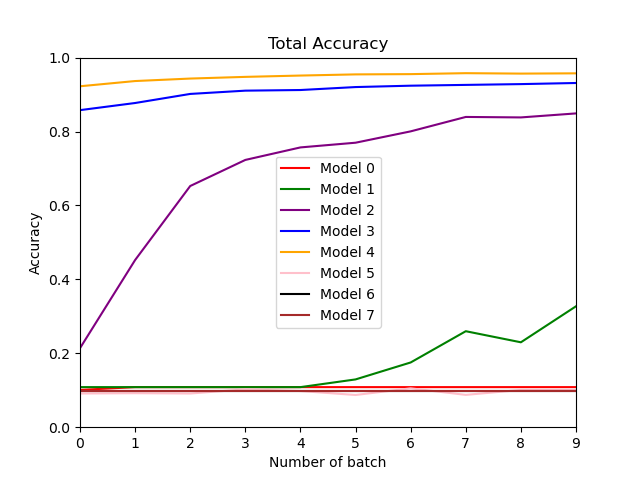
\includegraphics[width=.8\textwidth]{Fig_acc_p2_eta.png}\hfill
			\caption{Variation des performances pour $\eta$ variant de $1e^{-5}$ à $10$}	
		\end{figure*}
		
		Ici, chaque modèle est associé à un taux d'apprentissage de plus en plus grand à partir de $1e^{-5}$ (augmentation par $log(10)$). Les résultats indiquent que pour un taux d'apprentissage faible, i.e $1e^{-5}$ et $1e^{-4}$, le réseau ne dépasse pas $0.4$ de performance, comme c'est le cas pour un taux d'apprentissage important, i.e. $0.1$, $1$ et $10$. En outre, un taux compris entre $0.0001$, $0.001$, $0.01$ offre de belles performances, particulièrement pour $0.01$. Le modèle offrant le plus bel apprentissage est le numéro 2, même si ses performances finales sont inférieures. Cette valeur sera utilisée pour la suite de cette partie afin de voir si l'ajustement d'autres paramètres influencent la performance du réseau.\\		
		
	L'initialisation des \textbf{poids initiaux} est le deuxième paramètre dont l'influence tient à être quantifiée. Rappelons que le neurone reçoit des signaux en provenance de différentes sources (entrées) avec une certaine force associée (le poids), et plus cette valeur a de l'influence, plus l'intensité est forte, donc plus l'entrée correspondante l'est aussi. En ce qui concerne l'initialisation des poids, la littérature conseille de petites valeurs pour que le réseau s'ajuste au fur et à mesure des itérations.
	

		\begin{figure*}[!h]
			\centering
			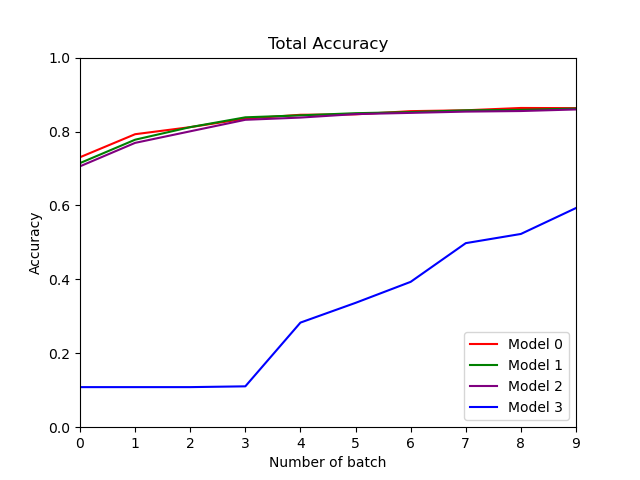
\includegraphics[width=.8\textwidth]{Fig_acc_p2_weight.png}\hfill
			\caption{Variation des performances pour différentes combinaisons de poids initiaux}	
		\end{figure*}

Ici, chaque modèle a reçu une initialisation de poids comme suit (c1 pour couche une et c2 pour couche 2): 
	
	\begin{enumerate}
	 \item Modèle 0 - c1 = 0.1, c2 = 0.1
	 \item Modèle 1 - c1 = 0.00001, c2 = 0.1
	 \item Modèle 2 - c1 = 0.1, c2 = 0.00001
	 \item Modèle 3 - c1 = 0.00001, c2 = 0.00001
	\end{enumerate}

	La seule remarque importante à fournir est que des poids initialisés trop faibles ne permettront pas d'atteindre de bonnes performances, en tout cas rapidement. Dans le cadre d'un réseau de neurones à une couche cachée, il suffit qu'une partie des poids soit initialement suffisamment élevée pour que l'algorithme converge rapidement vers de bonnes performances. Ici, les poids sont assignés en suivant la loi Uniforme sur l'intervalle spécifié. Il serait par la suite intéressant d'investiguer ces résultats pour des valeurs plus extrêmes et uniquement positives ou négatives.\\
	
	 \newpage
	Le dernier paramètre étudié dans cette partie est \textbf{le nombre de neurones} de la couche cachée. Les résultats sont les suivants ($\eta = 1e^{-3}$): 

		\begin{figure*}[!h]
			\centering
			\includegraphics[width=.8\textwidth]{Fig_acc_p2_size.png}\hfill
			\caption{Variation des performances pour le nombre de neurones pour la couchée cachée (respectivement, 64, 128, 256, $\eta = 1e^{-3}$)}	
		\end{figure*}
		
	Il est difficile ici de quantifier l'importance du nombre de neurones. Nous avons donc baisser le taux d'apprentissage, et les résultats sont plus saillants : un nombre élevé de neurone offre de meilleures performances. Il aurait été intéressant de fournir une visualisation pour un nombre de neurones beaucoup plus importants, mais faute de capacités suffisantes et du temps de traitement de l'algorithme, nous ne sommes pas aller au delà de 256.
	
		\begin{figure*}[!h]
			\centering
			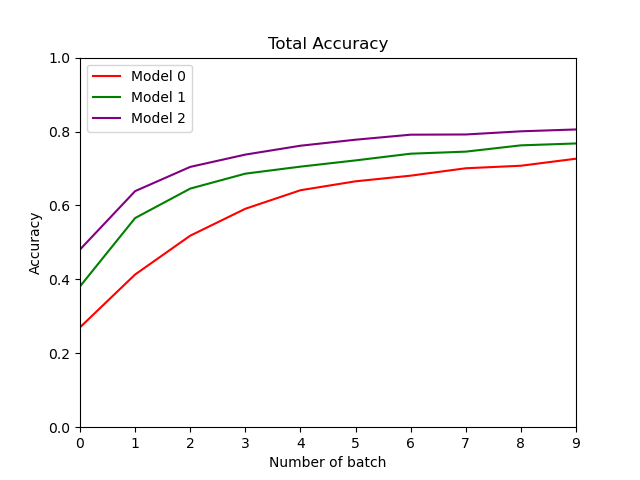
\includegraphics[width=.8\textwidth]{Fig_acc_p2_size_etavar.png}\hfill
			\caption{Variation des performances pour le nombre de neurones pour la couchée cachée (respectivement, 64, 128, 256, $\eta = 1e^{-4}$)}	
		\end{figure*}
	\newpage
		
		
	\section*{Partie III : Deep network}
	
	La partie II nous a permis d'identifier l'importance du \textbf{taux d'apprentissage}, spécifique au problème concerné (i.e. il n'y a pas de méthodes universelles permettant de déterminer le taux optimal). Dans le cadre d'un réseau avec une couche cachée, les performances du modèle peuvent varier énormément. Vis-à-vis des poids initiaux, l'influence semble moins importante. Enfin, un nombre important de neurone dans la couche cachée offre de meilleures performances.\\
	
	L'objectif de cette partie est tout d'abord d'observer l'influence de ces paramètres lors de \textbf{2 couches cachées}. Ensuite, de déterminer l'influence de \code{batch size}, de l'ajout d'une troisième couche cachée, et de la variation du nombre de neurones.
	
	Cette partie est accompagnée de la somme cumulée de la fonction de coût. Un bon modèle d'apprentissage devrait être associé à une fonction de coût dont la forme est logarithmique (augmente beaucoup au début puis se stabilise lors de l'arrivée à l'optimum).\\
	
	De la même manière que la partie II, cette première figure représente la performance du modèle en faisant varier le \textbf{taux d'apprentissage} $\eta$. Les résultats sont similairement les mêmes à la différence que les modèles les moins performants sont ceux situés aux valeurs extrêmes de $\eta$. La fonction de coût associée est cohérente avec la performance : les modèles 0 et 6 sont associés à une fonction de coût qui ne cesse d'augmenter, à l'inverse du modèle 4 et 5 qui se stabilisent.\\

		\begin{figure*}[!ht]
			\centering
			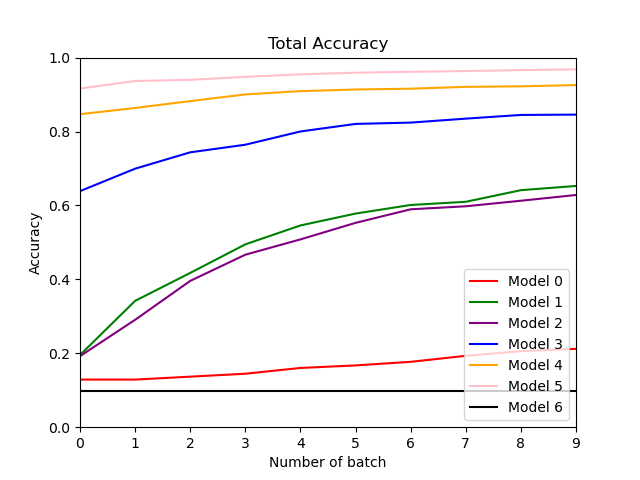
\includegraphics[width=.5\textwidth]{Fig_acc_p3.png}\hfill
			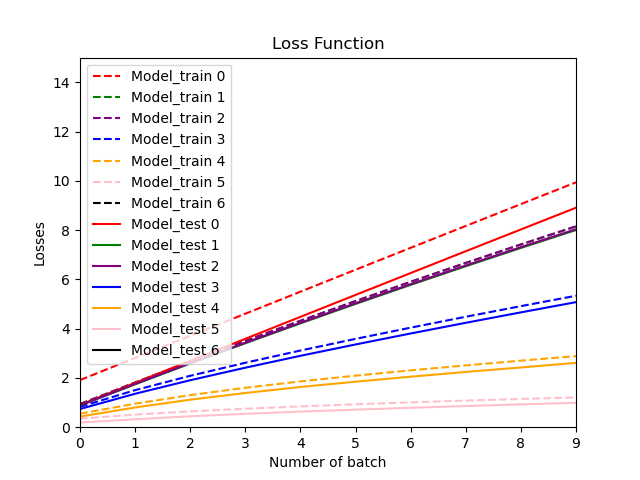
\includegraphics[width=.5\textwidth]{Fig_losses_p3.png}\hfill
			\caption{Variation des performances pour différentes valeurs de $\eta$}	
		\end{figure*}
		
	\newpage
	Pour les analyses suivantes, le modèle 3 associé à $\eta = e^{-3}$ a été sélectionné. Nous avons fait varier \textbf{les poids initiaux} des couches cachées de la façon suivante : les poids initialisés à $0.1$ pour toutes les couches, à $1e^{-4}$ pour toutes les couches, puis $1e^{-4}$ pour la première et troisième couche cachée avec la deuxième à $0.1$, et inversement pour le dernier modèle.
Les résultats sont cohérents avec ce qui a été observé précédemment : les poids initiaux ne doivent pas être trop petits. Ici, nous pouvons également émettre l'hypothèse que le plus important est l'initialisation des poids pour la première et troisième couche, la couche intermédiaire ne détermine pas, ou peu, les performances du modèle.\\
		
		\begin{figure*}[!ht]
			\centering
			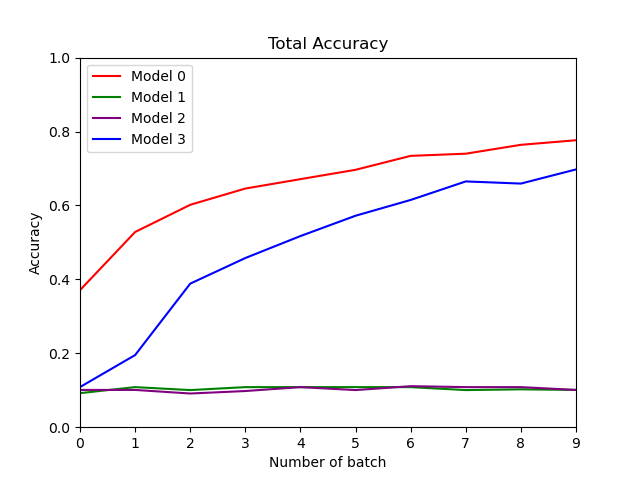
\includegraphics[width=.5\textwidth]{Fig_acc_p3_weight.png}\hfill
			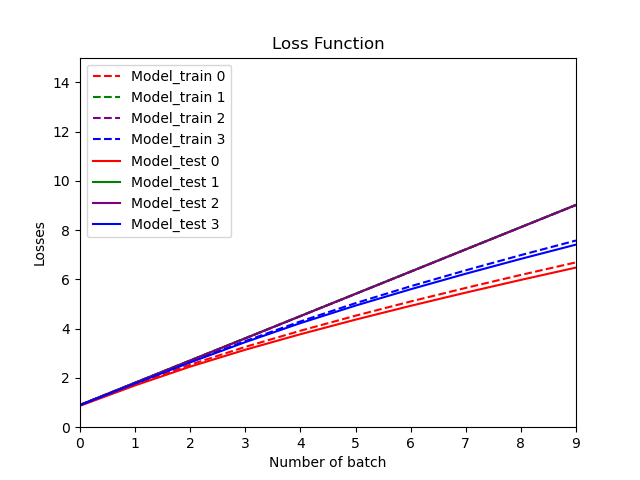
\includegraphics[width=.5\textwidth]{Fig_losses_p3_weight.png}\hfill
			\caption{Variation des performances par rapport aux poids initiaux}	
		\end{figure*}

	A présent, il est important de comprendre l'importance de \textbf{la taille du jeu de données d'apprentissage}. En ce sens, nous pourrions nous attendre à de meilleures performances des modèles ayant des jeux d'apprentissage plus élevés. Or, en faisant varier le nombre de \code{Batch Size} de 5 à 25, les différences frôlent le néant. La littérature souligne qu'une taille de lot élevée conduit souvent à des instabilités d'entraînement, au particulier au début, ce que nous ne notons pas particulièrement ici. La généralisation du modèle est également plus difficile, est Yann Lecun a même dit \textit{"Friends don't let friends use mini-batches larger than 32"}
	
		\begin{figure*}[!ht]
			\centering
			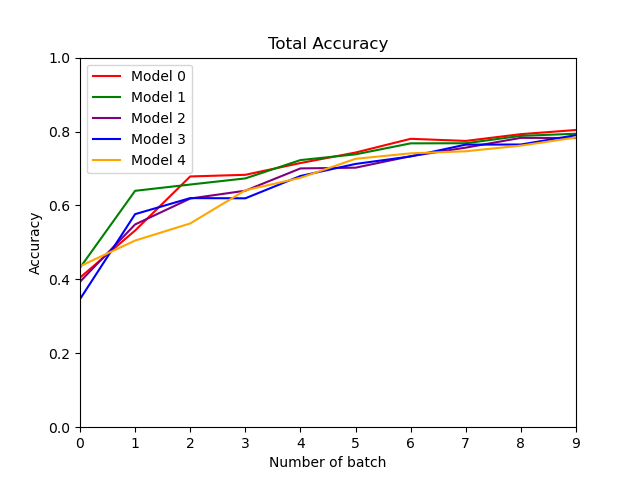
\includegraphics[width=.5\textwidth]{Fig_acc_p3_batchsize.png}\hfill
			\includegraphics[width=.5\textwidth]{Fig_losses_p3_batchsize.png}\hfill
			\caption{Variation des performances selon la taille de lot)}	
		\end{figure*}

	\newpage
	Les figures suivantes sont associées aux performances des modèles en faisant variant \textbf{le nombre de neurones par couche cachée}, respectivement : \textit{64 - 64, 256 - 256, 64 - 256} et inversement. D'après ces résultats, la deuxième couche cachée semble avoir le plus de poids parce qu'elle atteint les mêmes performance que le modèle 1, associé à un nombre de neurones élevés. Ces résultats sont intéressants mais il est nécessaire de comprendre l'implication de la première et dernière couche cachée lors de l'ajout d'une troisième couche cachée, intermédiaire.

		\begin{figure*}[!ht]
			\centering
			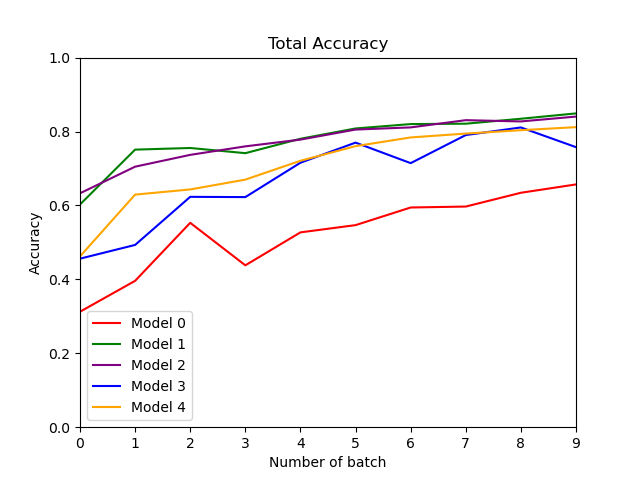
\includegraphics[width=.5\textwidth]{Fig_acc_p3_nb_neurons.png}\hfill
			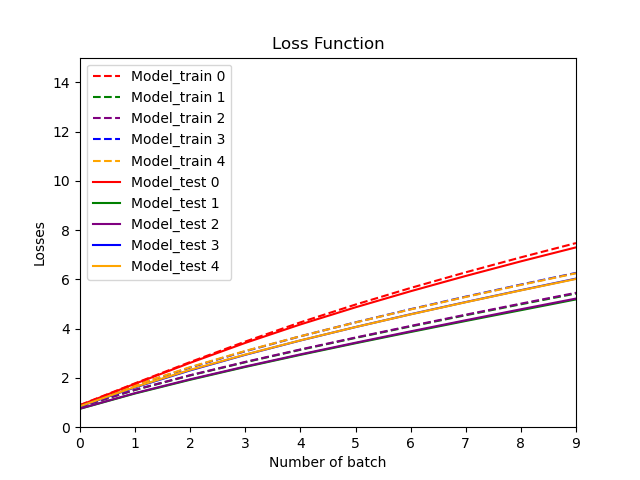
\includegraphics[width=.5\textwidth]{Fig_losses_p3_nb_neurons.png}\hfill
			\caption{Variation des performances selon le nombre de neurones par couche cachée}	
		\end{figure*}


Afin de quantifier l'influence du nombre de neurones par couches, nous avons ajouté une \textbf{troisième couche cachée} au modèle. La seule conclusion pouvant être émise ici est la nécessité d'un taux d'apprentissage supérieur lors de l'ajout de couches de neurones, en notant également que l'apprentissage semble très instable et sans convergence.\\

\textit{Caractéristiques : $\eta = 1e^-3$, pour chaque modèle : [256, 64, 64], [256, 128, 64], [256, 256, 64], [64, 64, 256], [64, 128, 156], [64, 256, 256].}

		\begin{figure*}[!ht]
			\centering
			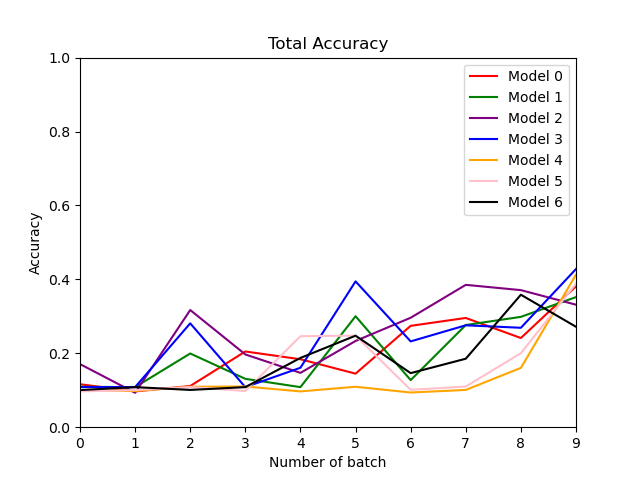
\includegraphics[width=.5\textwidth]{Fig_acc_p3_3C.png}\hfill
			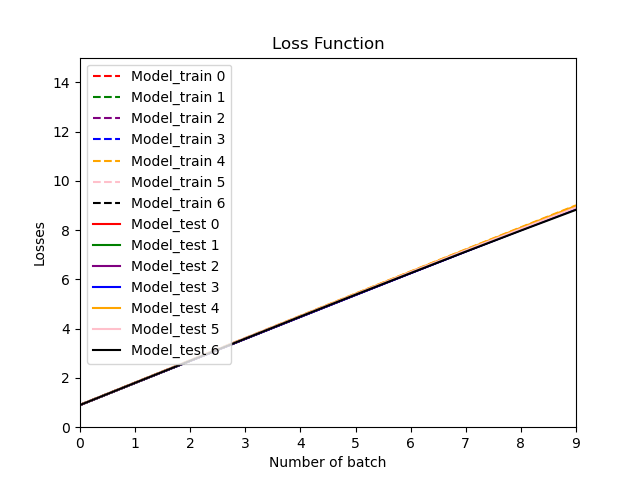
\includegraphics[width=.5\textwidth]{Fig_losses_3C.png}\hfill
			\caption{Variation des performances selon le nombre de neurones pour la couchée cachée, $\eta = 1e^-3$ }	
		\end{figure*}

	\newpage
	Nous avons donc augmenté le taux d'apprentissage, et la performance est plus importante. Néanmoins les modèles convergent tous vers la même performance, limitant encore la possibilité d'interpréter le comportement.\\
 		
\textit{Caractéristiques : $\eta = 1e^-2$, pour chaque modèle : [256, 64, 64], [256, 128, 64], [256, 256, 64], [64, 64, 256], [64, 128, 156], [64, 256, 256]. }

\begin{figure*}[!ht]
			\centering
			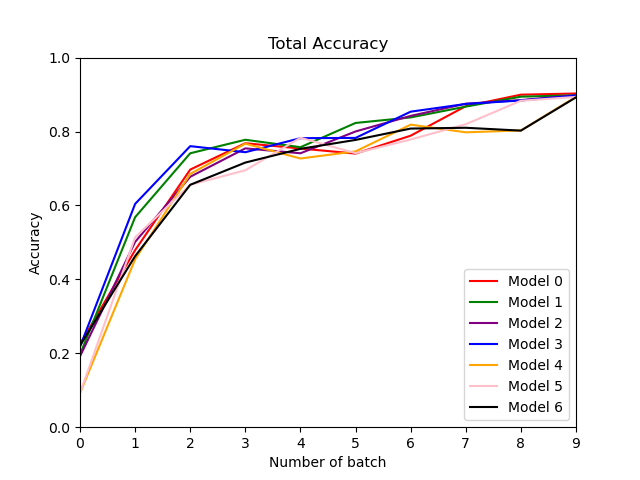
\includegraphics[width=.5\textwidth]{Fig_acc_p3_3C_eta.png}\hfill
			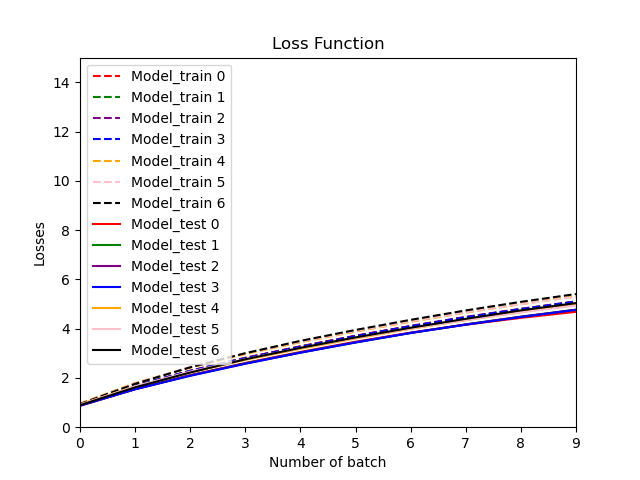
\includegraphics[width=.5\textwidth]{Fig_losses_p3_3C_eta.png}\hfill
			\caption{Variation des performances selon le nombre de neurones pour la couchée cachée, $\eta = 1e^-3$ }	
		\end{figure*}

	Nous avons donc \textbf{changé les combinaisons de nombre de neurones par couche} selon la logique suivante : un nombre élevé, intermédiaire et faible pour chaque couche, puis soit couche 1 et 3 élevées et 2 faible ou moyenne, soit des couches 1 et 3 faibles et une couche intermédiaire élevée. 

\textit{Caractéristiques : $\eta = 1e^-2$, pour chaque modèle : [256, 256, 256], [128, 128, 128], [64, 64, 64], [256, 64, 256], [256, 128, 256], [64, 256, 64]. }

		\begin{figure*}[!ht]
			\centering
			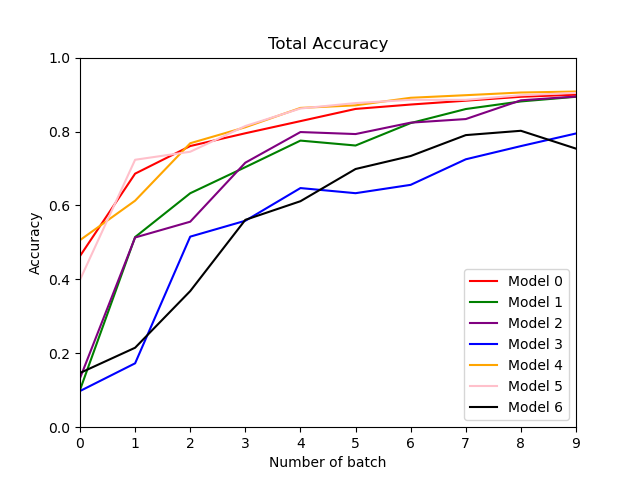
\includegraphics[width=.50\textwidth]{Fig_acc_p3_3C_v2.png}\hfill
			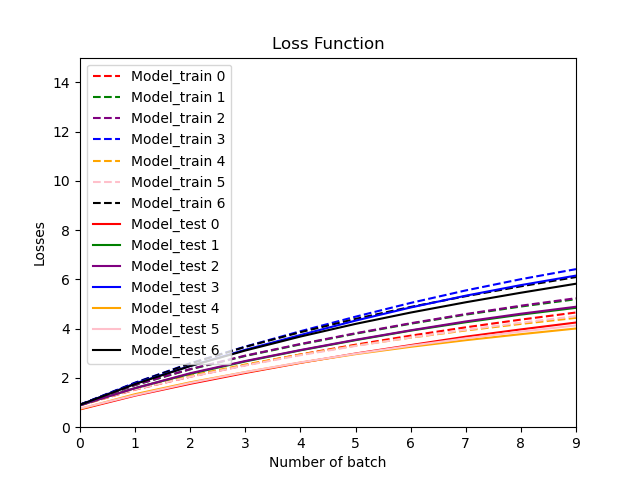
\includegraphics[width=.50\textwidth]{Fig_losses_p3_3C_v2.png}\hfill
			\caption{Variation des performances selon le nombre de neurones pour la couchée cachée, $\eta = 1e^-2$}	
		\end{figure*}

Les résultats sont clairs et semblent confirmer notre hypothèse de la partie 2 : un nombre de neurones élevé sur les couches périphériques offre de meilleurs résultats que pour un nombre élevé dans la couche intermédiaire. En effet, lors d'un nombre de neurones des couches cachées faibles, le réseau compresse l'information, et indéniablement, perd de l'information. A l'opposé, un nombre important de neurones dans les couches cachées améliore ses performances puisque cela augmente son nombre de paramètres, et donc ses capacités de généralisation. Néanmoins, un nombre trop important de neurones n'offre pas que des avantages, puisque cela augmente considérablement le temps de calcul, et parfois, amène au même résultat qu'un faible nombre de neurones, certainement par une redondance des paramètres. 


	\section*{Partie IV : Pour aller plus loin}
	Nous avons décidé de nous intéresser à l'influence des \textbf{fonctions d'activation} dans le cadre d'un réseau à deux couches cachées. Nous avons fait varier le taux d'apprentissage pour chaque modèle. Les figures suivantes indiquent de meilleures performances pour la fonction d'activation ReLU pour $\eta = 0.01$. Néanmoins, les modèles semblent sur-ajustés, et perdent potentiellement en capacité de généralisation.
	
		\begin{figure*}[!ht]
			\centering
			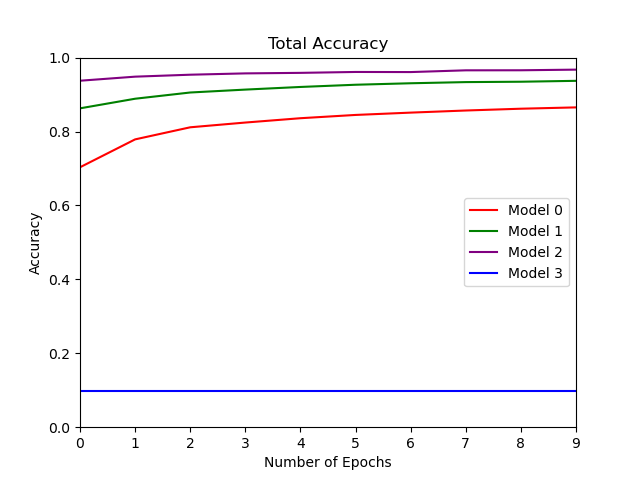
\includegraphics[width=.5\textwidth]{Fig_p4_acc_tanh.png}\hfill
			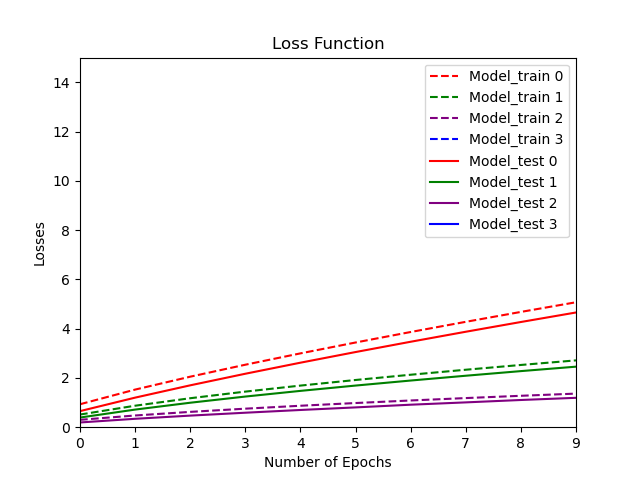
\includegraphics[width=.5\textwidth]{Fig_p4_losses_tanh.png}\hfill
			\caption{Variation des performances selon la fonction d'activation Tanh}	
		\end{figure*}
		
		\begin{figure*}[!ht]
			\centering
			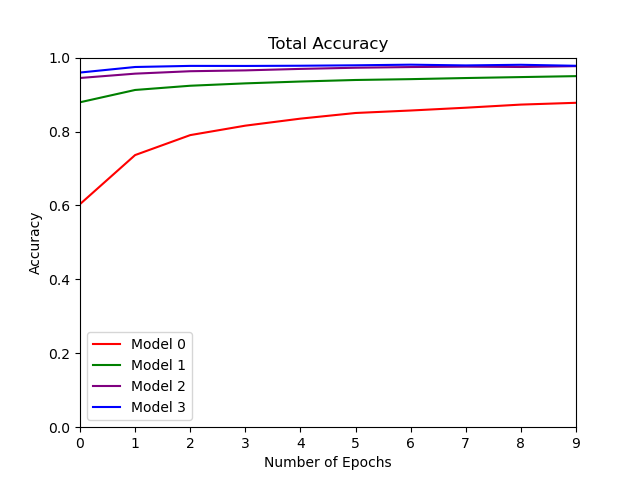
\includegraphics[width=.5\textwidth]{Fig_p4_relu.png}\hfill
			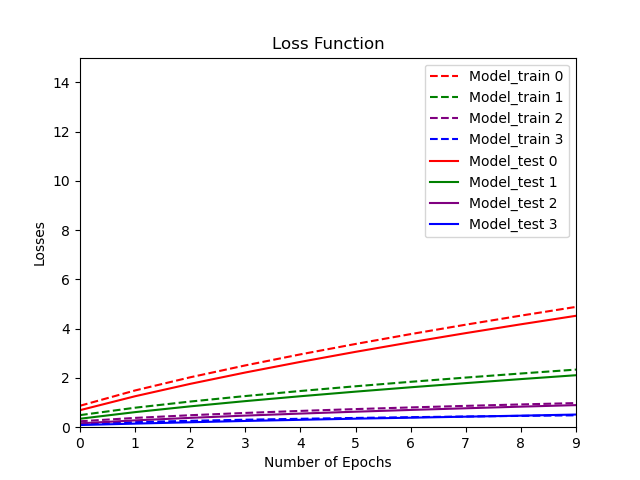
\includegraphics[width=.5\textwidth]{Fig_p4_losses_relu.png}\hfill
			\caption{Variation des performances selon la fonction d'activation ReLU}	
		\end{figure*}
		
		\begin{figure*}[!ht]
			\centering
			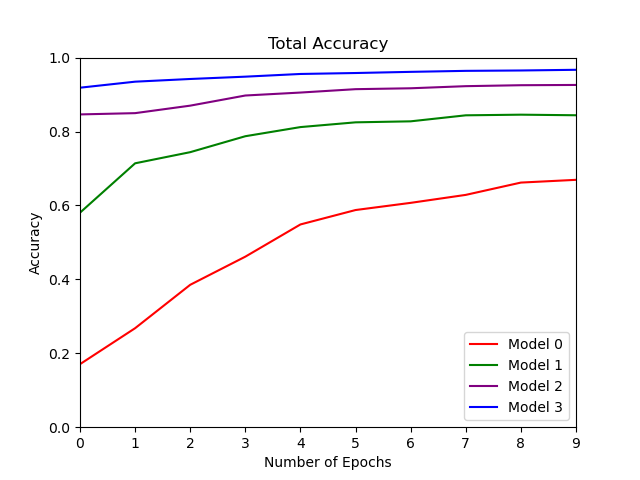
\includegraphics[width=.5\textwidth]{Fig_p4_acc_sigmoid.png}\hfill
			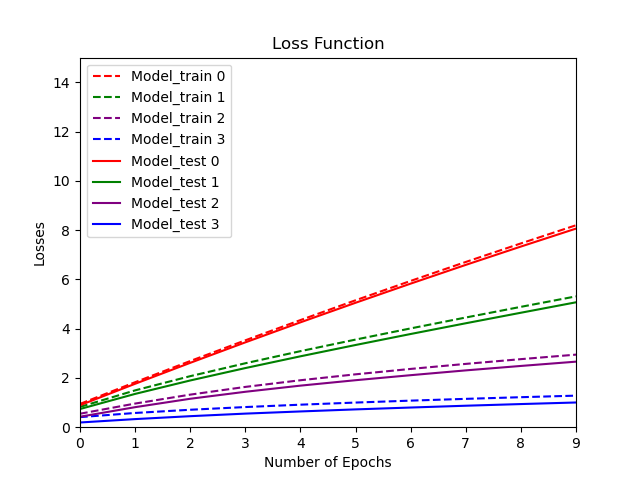
\includegraphics[width=.5\textwidth]{Fig_p4_losses_sigmoid.png}\hfill
			\caption{Variation des performances selon la fonction d'activation Sigmoid}	
		\end{figure*}
		
		\newpage
		Pour finir, nous avons testé \textbf{une initialisation des poids selon une loi normale}. Les résultats sont les suivants : 
		\begin{figure*}[!ht]
			\centering
			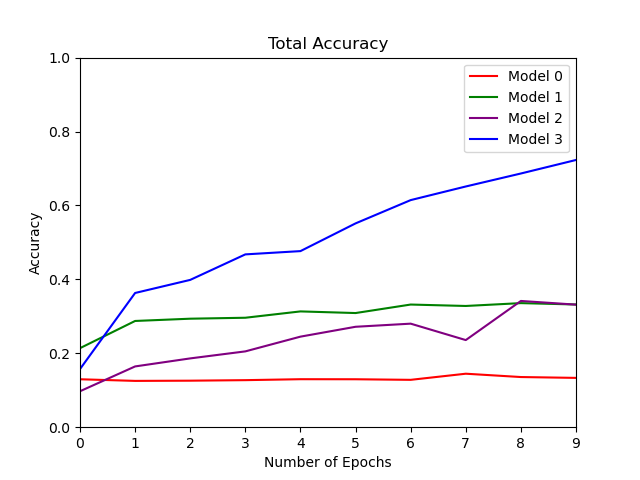
\includegraphics[width=.5\textwidth]{Fig_p4_acc_gauss.png}\hfill
			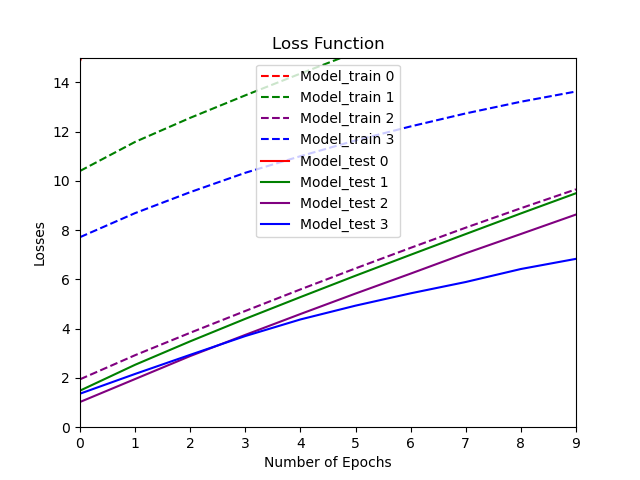
\includegraphics[width=.5\textwidth]{Fig_p4_losses_goss.png}\hfill
			\caption{Variation des performances selon une initialisation gaussienne des poids}	
		\end{figure*}
		
		C'est la première fois, durant l'ensemble des variations des paramètres, que nous observons une telle différence entre la fonction de coût d'apprentissage et de test. Vis-à-vis de la performance, nous arrivons à la même conclusion que précédemment : le taux d'apprentissage est le paramètre le plus important.
\end{document}